\documentclass[11pt]{article}
\usepackage[margin=1in]{geometry}
\usepackage{amsmath,amssymb,amsthm}
\usepackage{graphicx}
\usepackage{hyperref}
\usepackage{setspace}
\usepackage{float}

\setlength{\parskip}{0.75em}
\setlength{\parindent}{0pt}

\title{Radioactive Decay And Isochron Dating of Moon Rocks}
\author{Dave Rosenman}
\date{December 5, 2017}

\begin{document}

\maketitle

by Dave Rosenman

The rate of decay of a sample of a radioactive isotope is proportional to the number, $N$, of particles of that isotope. Mathematically, this can be represented as

\begin{equation}
\frac{dN(t)}{dt} = -\lambda N(t)
\end{equation}

Equation (1) is a simple first order differential equation. It can be solved as follows. First, divide both sides of (1) by $N(t)$:

\[
\frac{1}{N(t)}\frac{dN(t)}{dt} = -\lambda
\]

Since,

\begin{equation}
\frac{d}{dt}\left[\ln(N(t))\right]
=
\frac{d}{dN}\left[\ln(N(t))\right]\frac{dN(t)}{dt}
=
\frac{1}{N(t)}\frac{dN(t)}{dt}
=
-\lambda
\end{equation}

Next, integrate both sides of equation (2):

\begin{equation}
\int_{{t_0}}^t {\underbrace {\frac{d}{{dt}}\left[ {\ln \left( {N\left( t \right)} \right)} \right]}_{\frac{1}{{N\left( t \right)}}\frac{{dN\left( t \right)}}{{dt}}}dt}  =  - \int_{{t_0}}^t {\lambda t} 
\end{equation}

Apply the fundamental theorem of calculus to both sides of equation (3). The integral on the left side is equal to

\begin{equation}
\ln(N(t)) - \ln(N(t_0))
=
\ln\!\left(\frac{N(t)}{N(t_0)}\right)
\end{equation}

And, since $\lambda$ is a constant, the integral on the right side of equation (3) is equal to

\begin{equation}
-\int_{t_0}^{t}\lambda\,dt = -\lambda (t-t_0)
\end{equation}

Letting $N(t)=N$, $t_0=0$, and $N_0=N(t_0)=N(t=0)$, from (3), (4), and (5):

\[
\ln\!\left(\frac{N}{N_0}\right)=-\lambda t
\]

\[\underbrace {{e^{\ln \left( {\frac{N}{{{N_0}}}} \right)}}}_{N/{N_0}} = {e^{ - \lambda t}}\]

\[
\frac{N}{N_0}=e^{-\lambda t}
\]

\begin{equation}
N = N_0 e^{-\lambda t}
\end{equation}

\begin{equation}
t = -\frac{1}{\lambda}\ln\!\left(\frac{N}{N_0}\right)
\end{equation}

If we define the half life of the radioactive isotope, the time it takes for half of the sample to decay, as $t_{1/2}$, we can solve for the decay constant $\lambda$ in terms of the half life:

\[
N(t_{1/2}) = \frac{N_0}{2} = N_0 e^{-\lambda t_{1/2}}
\]

\[
\frac{1}{2}=e^{-\lambda t_{1/2}}
\]

\[
e^{\lambda t_{1/2}}=2
\]

\[
\ln\!\left(e^{\lambda t_{1/2}}\right)=\ln(2)
\]

\[\underbrace {\ln \left( {{e^{\lambda {t_{1/2}}}}} \right)}_{\lambda {t_{1/2}}} = \ln \left( 2 \right)\]

\begin{equation}
\boxed{\lambda = \frac{\ln(2)}{t_{1/2}}}
\end{equation}

The value of $\lambda$ can be determined by experimentally measuring the half-life of the radioactive isotope. Assuming that the half life of a radioactive isotope is in fact constant (and therefore $\lambda$ is a constant), we are still faced with a problem. Let’s assume that we have discovered rocks that we believe formed at the same time. If we want to date each of the rocks using equation (7), it appears that unless we know $N_0$, the number of particles a radioactive isotope present in the rock at its formation, even if $\lambda$ is a constant, we’ll have no way to determine the age of the rock. Making matters worse, it appears that there is no way of determining whether or not the rocks in question are ``closed'' systems. If the ``system'' (the rock in question) has been a closed system since its formation, that means that no material has been added or removed from the rock since its formation.

So is there no way to determine the age of rocks from radioactive isotopes present in the rocks? No. There are multiple possible methods for determining the age of rocks. The method I will focus on is the rubidium--strontium isochron method.

There are two naturally occurring isotopes of rubidium. $^{87}\mathrm{Rb}$ is a radioactive isotope of rubidium, and has half life of $4.8$ billion years. $^{85}\mathrm{Rb}$ is a stable isotope of rubidium.\footnote{$^{87}\mathrm{Rb}$ decays to $^{87}\mathrm{Sr}$ via beta decay (one of $^{87}\mathrm{Rb}$ decays into a proton, an electron, and an antineutrino).}

\[
{}^{87}_{37}\mathrm{Rb}
\rightarrow
{}^{87}_{38}\mathrm{Sr}
+
{}^{0}_{-1}\beta
\]

Strontium--87 and Strontium--86 are two stable isotopes of strontium. If a group of rocks are co-genetic, meaning they are formed at the same time and place and are derived from the same parent material, they will have the same ratio of
\[
\frac{^{87}\mathrm{Sr}}{^{86}\mathrm{Sr}}
\]
when they are formed.\footnote{Assuming that the rocks are closed systems, the amount of $^{86}\mathrm{Sr}$ at the time of the rocks should be the same today as when the rocks were formed, since $^{86}\mathrm{Sr}$ is not produced by radioactive decay. The amount of $^{87}\mathrm{Sr}$ in each rock at the time of formation should be different from the amount of $^{87}\mathrm{Sr}$ in each rock today, since $^{87}\mathrm{Sr}$ can form from the decay of $^{87}\mathrm{Rb}$.}

If a rock has been a closed system since its time of formation, each $^{87}\mathrm{Rb}$ particle that decays forms a single $^{87}\mathrm{Sr}$ particle. So the amount of $^{87}\mathrm{Sr}$ particles measured long after the rock has formed is

\begin{equation}
\left(^{87}\mathrm{Sr}\right)_{\mathrm{final}}
=
\left(^{87}\mathrm{Sr}\right)_{\mathrm{initial}}
+
\left[\left(^{87}\mathrm{Rb}\right)_{\mathrm{initial}}-\left(^{87}\mathrm{Rb}\right)_{\mathrm{final}}\right]
\end{equation}

Since the amount of $^{86}\mathrm{Sr}$ is assumed to be constant, it follows that

\begin{equation}
\left(\frac{^{87}\mathrm{Sr}}{^{86}\mathrm{Sr}}\right)_{\mathrm{final}}
=
\left(\frac{^{87}\mathrm{Sr}}{^{86}\mathrm{Sr}}\right)_{\mathrm{initial}}
+
\frac{1}{^{86}\mathrm{Sr}}
\left[
\left(^{87}\mathrm{Rb}\right)_{\mathrm{initial}}
-
\left(^{87}\mathrm{Rb}\right)_{\mathrm{final}}
\right]
\end{equation}

From equation (6), letting $N=\left(^{87}\mathrm{Rb}\right)_{\mathrm{final}}$ and $N_0=\left(^{87}\mathrm{Rb}\right)_{\mathrm{initial}}$:

\[
\left(^{87}\mathrm{Rb}\right)_{\mathrm{final}}
=
\left(^{87}\mathrm{Rb}\right)_{\mathrm{initial}}e^{-\lambda t}
\]

\[
\left(^{87}\mathrm{Rb}\right)_{\mathrm{final}}e^{\lambda t}
=
\left(^{87}\mathrm{Rb}\right)_{\mathrm{initial}}
\]

\begin{equation}
\left(^{87}\mathrm{Rb}\right)_{\mathrm{initial}}
-
\left(^{87}\mathrm{Rb}\right)_{\mathrm{final}}
=
\left(^{87}\mathrm{Rb}\right)_{\mathrm{final}}\left(e^{\lambda t}-1\right)
\end{equation}

From (10) and (11) it follows that

\begin{equation}
\left(\frac{^{87}\mathrm{Sr}}{^{86}\mathrm{Sr}}\right)_{\mathrm{final}}
=
\left(\frac{^{87}\mathrm{Sr}}{^{86}\mathrm{Sr}}\right)_{\mathrm{initial}}
+
\frac{\left(^{87}\mathrm{Rb}\right)_{\mathrm{final}}}{^{86}\mathrm{Sr}}
\left(e^{\lambda t}-1\right)
\end{equation}

We are assuming that all of the rocks collected formed at the same time and thus are the same age. We are assuming that
\[
\left(\frac{^{87}\mathrm{Sr}}{^{86}\mathrm{Sr}}\right)_{\mathrm{initial}}
\]
is the same for all rocks in our sample (since we assume they formed at the same time),
\[
\left(\frac{^{87}\mathrm{Sr}}{^{86}\mathrm{Sr}}\right)_{\mathrm{final}}
\]
depends on the initial amount of $^{87}\mathrm{Sr}$, $^{86}\mathrm{Sr}$, and the amount of $^{87}\mathrm{Rb}$ present at the time of formation (which will vary from rock to rock),
\[
\frac{\left(^{87}\mathrm{Rb}\right)_{\mathrm{final}}}{^{86}\mathrm{Sr}}
\]
depends on both the amount of $^{87}\mathrm{Rb}$ at the time of formation and the initial amount of $^{86}\mathrm{Sr}$ present at the time of formation, which will vary from rock to rock. From these assumptions, including the assumption that the half life of $^{87}\mathrm{Rb}$ is a constant that has not changed over time (and is independent of geological conditions), equation (12) has the form of a simple linear equation.

\begin{equation}
\underbrace{\left(\frac{^{87}\mathrm{Sr}}{^{86}\mathrm{Sr}}\right)_{\mathrm{final}}}_{y}
=
\underbrace{\left(\frac{^{87}\mathrm{Sr}}{^{86}\mathrm{Sr}}\right)_{\mathrm{initial}}}_{b}
+
\underbrace{\frac{\left(^{87}\mathrm{Rb}\right)_{\mathrm{final}}}{^{86}\mathrm{Sr}}}_{x}
\underbrace{\left(e^{\lambda t}-1\right)}_{m}
\end{equation}

So if we collect a sample of rocks that we assume were formed at the same time and place, by the same parent material, measure the ratios of $^{87}\mathrm{Rb}$ to $^{86}\mathrm{Sr}$ and $^{87}\mathrm{Sr}$ to $^{86}\mathrm{Sr}$ present in each rock, a graph of
\[
\left(\frac{^{87}\mathrm{Sr}}{^{86}\mathrm{Sr}}\right)_{\mathrm{final}}
\]
(the ratio of $^{87}\mathrm{Rb}$ to $^{86}\mathrm{Sr}$ versus $^{87}\mathrm{Sr}$ to $^{86}\mathrm{Sr}$) should form a straight line. The slope of that line will be $(e^{\lambda t}-1)$ and the $y$-intercept will give us the initial ratio of $^{87}\mathrm{Sr}$ to $^{86}\mathrm{Sr}$.

We have made multiple assumptions, and these can all be tested by plotting the ratio of $^{87}\mathrm{Rb}/^{86}\mathrm{Sr}$ versus $^{87}\mathrm{Sr}/^{86}\mathrm{Sr}$. If we find a linear relationship between $^{87}\mathrm{Rb}/^{86}\mathrm{Sr}$ and $^{87}\mathrm{Sr}/^{86}\mathrm{Sr}$, we can be confident that our assumptions were correct.

The following data set is of moon rocks collected during the Apollo 17 mission. The relationship between $^{87}\mathrm{Rb}/^{86}\mathrm{Sr}$ and $^{87}\mathrm{Sr}/^{86}\mathrm{Sr}$ forms nearly a perfect straight line.\footnote{The dataset can be downloaded  \href{https://github.com/DRosenman/advanced-experimental-physics/blob/master/graphs/moonrockdating/apollo17_moon_rock_data.csv}{here}.}

\begin{figure}[H]
    \centering
    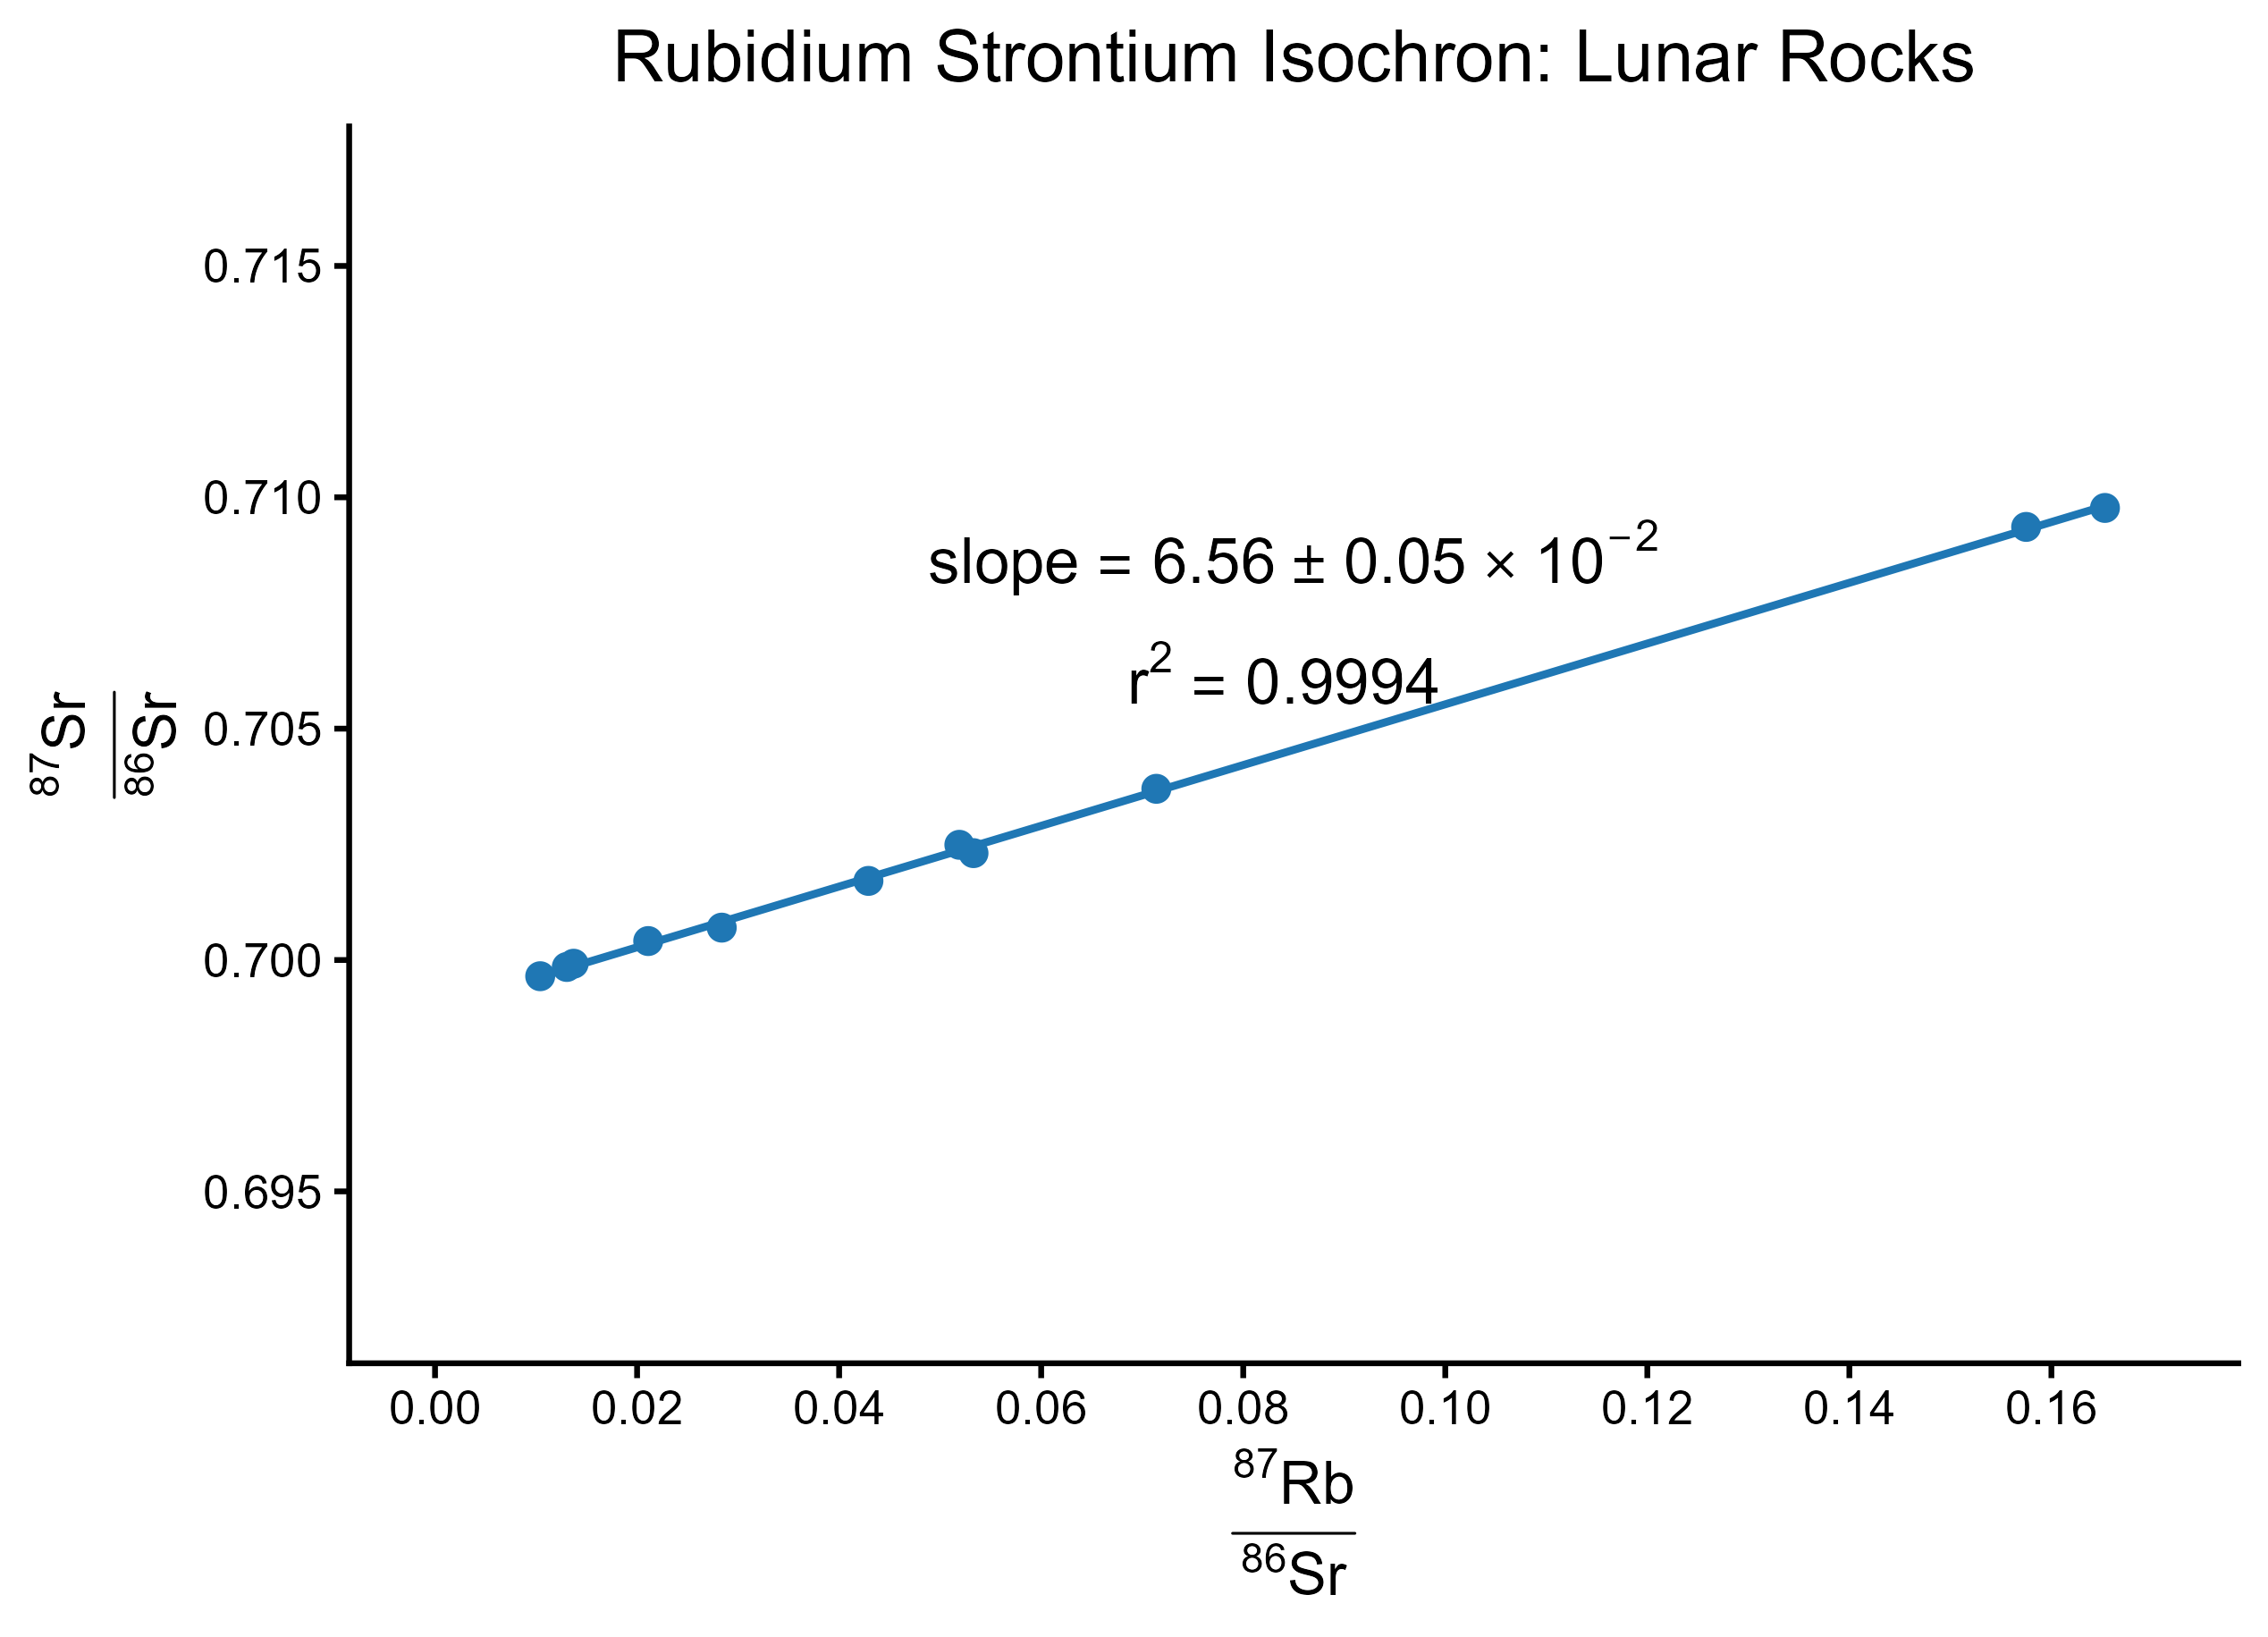
\includegraphics[width=0.85\textwidth]{graphs/moonrockdating/rb_sr_isochron_plot.png}
    \caption{Rubidium--strontium isochron plot for Apollo 17 lunar rock samples. The slope of the best-fit line is used to estimate the age of the rocks.}
    \label{fig:moonrockdating}
\end{figure}

The slope of the best-fit line is $m = 6.56 \times 10^{-2}$. From equation (13):

\[
m=e^{\lambda t}-1
\]

\[
e^{\lambda t}=m+1
\]

\[
\lambda t=\ln(m+1)
\]

\begin{equation}
t=\frac{1}{\lambda}\ln(m+1)
\end{equation}

From equation (8), equation (14), and the fact that the measured half life of $^{87}\mathrm{Rb}$ is $48$ billion years:

\begin{equation}
t
=
\frac{t_{1/2}}{\ln(2)}\ln(m+1)
=
\frac{48.8\times10^9 \ln(6.56\times10^{-2}+1)}{\ln(2)}
\end{equation}

\[
t = 4.47 \text{ billion years}
\]

The moon rocks that the Apollo 17 collected are approximately $4.5$ billion years old.

\section*{Notes}

\begin{enumerate}
    \item Dating Rocks with the Rb--Sr ``Isochron'' Method\\
    \url{http://www.sciencecourseware.org/VirtualDating/DatingDemo/files/50RbSr.html}

    \item The Rubidium--Strontium System\\
    \url{http://www.emufor.br/air/wp-content/uploads/2014/03/Geochronology__2008__02__Rb-Sr.pdf}

    \item ``Rb-Sr study of a lunar dunite and evidence for early lunar differentiation,'' Papanastassiou, D. A. \& Wasserburg, G. J.\\
    \url{http://adsbit.harvard.edu/full/1975LPSC....6.1467P/0001467.000.html}
\end{enumerate}

\end{document}